%=======================02-713 LaTeX template, following the 15-210 template==================
%
% You don't need to use LaTeX or this template, but you must turn your homework in as
% a typeset PDF somehow.
%
% How to use:
%    1. Update your information in section "A" below
%    2. Write your answers in section "B" below. Precede answers for all 
%       parts of a question with the command "\question{n}{desc}" where n is
%       the question number and "desc" is a short, one-line description of 
%       the problem. There is no need to restate the problem.
%    3. If a question has multiple parts, precede the answer to part x with the
%       command "\part{x}".
%    4. If a problem asks you to design an algorithm, use the commands
%       \algorithm, \correctness, \runtime to precede your discussion of the 
%       description of the algorithm, its correctness, and its running time, respectively.
%    5. You can include graphics by using the command \includegraphics{FILENAME}
%
\documentclass[11pt]{article}
\usepackage{amsmath,amssymb,amsthm}
\usepackage{graphicx}
\usepackage[margin=1in]{geometry}
\usepackage{fancyhdr}
\setlength{\parindent}{0pt}
\setlength{\parskip}{5pt plus 1pt}
\setlength{\headheight}{13.6pt}
\usepackage{algorithm}
\usepackage{algpseudocode}
\usepackage{float}

\newcommand*{\permcomb}[4][0mu]{{{}^{#3}\mkern#1#2_{#4}}}
\newcommand*{\perm}[1][-3mu]{\permcomb[#1]{P}}
\newcommand*{\comb}[1][-1mu]{\permcomb[#1]{C}}

\newcommand\question[2]{\vspace{.25in}\hrule\textbf{#1: #2}\vspace{.5em}\hrule\vspace{.10in}}
\renewcommand\part[1]{\vspace{.10in}\textbf{(#1)}}
\newcommand\algorithmcode{\vspace{.10in}\textbf{Algorithm: }}
\newcommand\correctness{\vspace{.10in}\textbf{Correctness: }}
\newcommand\runtime{\vspace{.10in}\textbf{Running time: }}
\pagestyle{fancyplain}
\lhead{\textbf{\NAME\ (\ANDREWID)}}
\chead{\textbf{HW\HWNUM}}
\rhead{CSE 836, \today}

\begin{document}\raggedright
%Section A==============Change the values below to match your information==================
\newcommand\NAME{Nan Du}  % your name
\newcommand\ANDREWID{dunan}     % your andrew id
\newcommand\HWNUM{2}              % the homework number
%Section B==============Put your answers to the questions below here=======================

% no need to restate the problem --- the graders know which problem is which,
% but replacing "The First Problem" with a short phrase will help you remember
% which problem this is when you read over your homeworks to study.

\question{1}{simulated PacBio reads} 

\part{a} 

To estimate a reasonable k, we can follow the method section in MHAP paper. So the expected number of kmer $ E[X_c] $ can be calculated use following equation:

\[ E[X_c] = (P_{ovl} - P_{ovl} P_{rand})M + P_{rand}L \]

M is the size of overlap part and L is the length of the read. $ P_{ovl} $ and $ P_{rand} $ are given by following equation:

\[ P_{rand} = 1 - (1 - |\varSigma|^{-k})^{K} \]
\[ P_{ovl} = [(1-\varepsilon)^{2}+\varepsilon^{2}\frac{1}{|\varSigma| - 1}]^{k} \]

K is the number of kmers in the read, we can assume is equal to the length of read, $ \varepsilon $ is the error rates.

From this calculation, we found that when $ k = 16 $, usually we can only expect several kmers. For our MinHash sampling process,I think the k = 16 is too large. I tried with $ k = 10 $ and $ k = 12 $, as the expected number of matches is much higher.

For number of permutations, I believed the reasonable value should be proportional to the read length. Given the thousands of bases in Pacbio Reads, I think $ m = 512 $ and $ m = 1024 $ are reasonable choices.

I was trying to follow the code that use false positive rate and false negative rate to optimize the number of r, but it always returns 1, so right now in my experiment the r always be 1.

Jaccardi similarity threhold is determined by a small scale test, I found for most overlapped reads, the similarity for 10-mer is only 0.01-0.10 level. So I choose 0.01 as my threshold. I also use 0.04 threshold which is given from MHAP paper。

For 30X dataset:
\begin{enumerate}
\item
k=10 1024 0.01\\
116444191 pairs passed the filters\\
sensitivity 0.9782145414156769\\
FPR 0.8314137831129967\\
accuracy 0.0040011012657557125\\
F1 0.007969605185993432\\

\item
k=10 1024 0.04
9722271 pairs passed the filters\\
sensitivity 0.4537027511070146\\
FPR 0.06814697975590785\\
accuracy 0.022226288487535474\\
F1 0.04237660405124178\\

\item
k = 12 1024 0.01\\
26040512 pairs passed the filters
sensitivity 0.8414108477978336\\
FPR 0.18380383018735438\\
accuracy 0.015389405553930736\\
F1 0.03022597793028742\\
\end{enumerate}

For 20X dataset:
\begin{enumerate}
	\item
	k=10 1024 0.04\\
	5201162 pairs passed the filters\\
	sensitivity 0.3249885241959911\\
	FPR 0.008208450660925973\\
	accuracy 0.04001951871524094\\
	F1 0.07126354927725775\\
	
	\item
	k = 12 1024 0.01\\
	38755561 pairs passed the filters\\
	sensitivity 0.7990532071359203\\
	FPR 0.06287228961496219\\
	accuracy 0.013205227502705998\\
	F1 0.025981089114060423\\
\end{enumerate}

From the above result, I believed k = 12 with 0.01 threshold is more reasonable for our filter task. k= 10 with 0.01 threshold has too many false positive pass our filter. And k = 10 with 0.04 has a lot of false negative situations.

\part{b}

For the memory usage (30X dataset):

\begin{center} 
	\begin{tabular}{ | l | l | l | l | l |} 
		\hline k & m & threshold & memory & running time \\ 
		\hline 10 & 1024 & 0.04 & 3354296kb & 03:10:37 \\ 
		\hline 10 & 512 & 0.01 & 832444kb & 03:16:16 \\ 
		\hline 10 & 1024 &0.01 & 1235856kb & 03:16:26 \\ 
		\hline 12 & 1024 &0.01 & 1401860kb & 03:51:17\\ 
		\hline 
	\end{tabular} 
\end{center}

\part{c}

\begin{figure}[H]
\centering
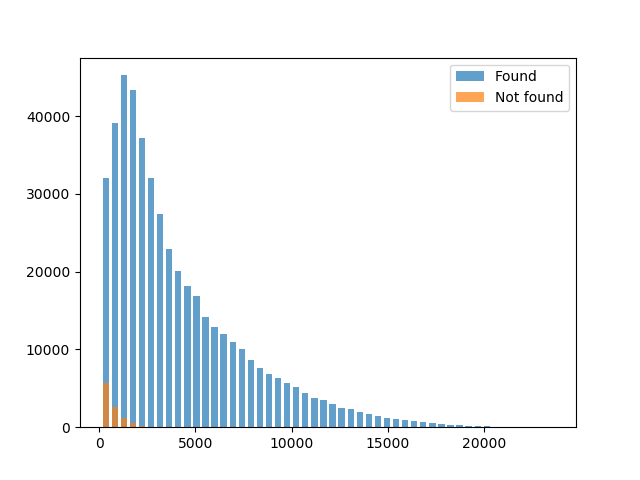
\includegraphics[width = .8\textwidth]{Ecoli_Pacbio_simulate_30X_k10_1024_0p01.png}
\caption{Overlap size distribution for k =10 with 1024 permutations and 0.01 threshold}
\label{fig1}
\end{figure}

\begin{figure}[H]
	\centering
	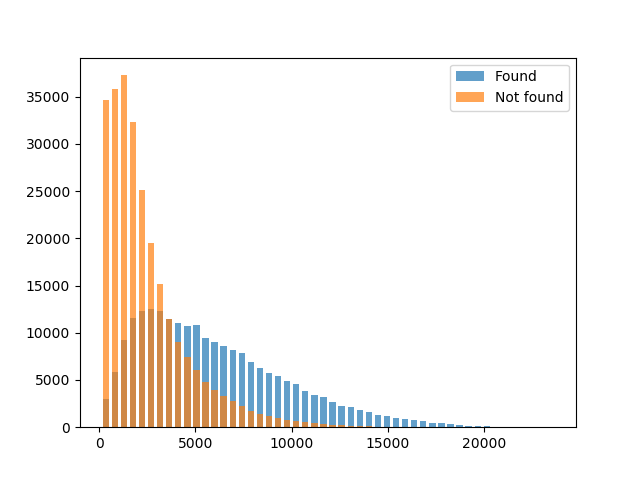
\includegraphics[width = .8\textwidth]{Ecoli_Pacbio_simulate_30X_k10_1024_0p04.png}
	\caption{Overlap size distribution for k =10 with 1024 permutations and 0.04 threshold}
	\label{fig2}
\end{figure}

\begin{figure}[H]
	\centering
	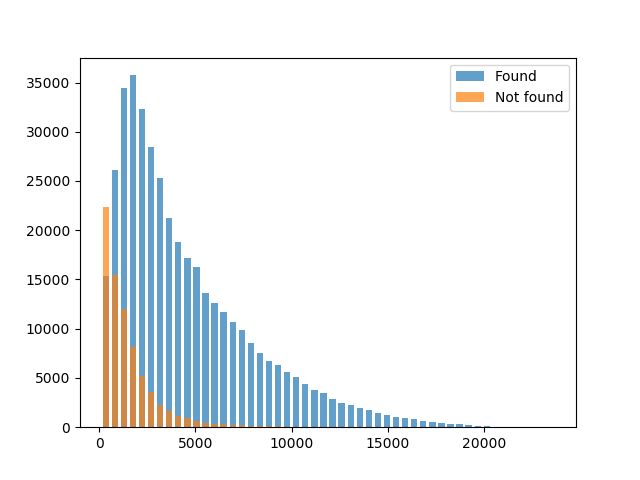
\includegraphics[width = .8\textwidth]{Ecoli_Pacbio_simulate_30X_k12_1024_0p01.png}
	\caption{Overlap size distribution for k =12 with 1024 permutations and 0.01 threshold}
	\label{fig3}
\end{figure}

Generally speaking, most overlap pairs we are missing have smaller overlap size compared to those we reported.

And when we decrease the threshold, we can find that more overlap pairs with smaller overlap size will be included in our final reported results.

\question{2}{simulated viral metagenomics}

For this dataset, I followed the suggestions that if several reads are hashing to one bucket in LSH, then they are treated as one cluster. So the expected number of clusters is mainly determined by the choices of k, hashing function, and number of permutations(but seems this not really change anything in my experiment).

So I determine the properties of cluster by major vote from the reads in the cluster. If there are more reads from HCV, then I believe this cluster should belong to HCV, and all reads from HGV or HIV will be treated as error. By doing this I can made a confusion matrix for each experiment.

I also attached the cluster result for k = 10 in handin. Each line is a single cluster in the file.

\part{a}

I found the most important parameters is the size of kmer.
\begin{enumerate}
	\item 
	
	\begin{figure}[H]
		\centering
		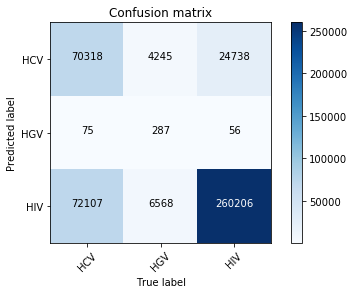
\includegraphics[width = .5\textwidth]{cm_k6.png}
		\caption{Confusion Matrix with k = 6}
		\label{fig4}
	\end{figure}
For k = 6:\\
	For 438601 reads we generate 1358 clusters\\
	70.81\% HCV reads classfied into right clusters (HCV dominated cluster)\\
	68.66\% HGV reads classfied into right clusters (HGV dominated cluster)\\
	76.78\% HIV reads classfied into right clusters (HIV dominated cluster)\\
	
	\item 
	
	\begin{figure}[H]
		\centering
		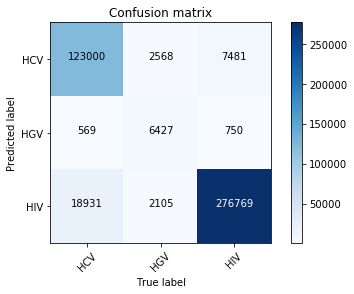
\includegraphics[width = .5\textwidth]{cm_k8.png}
		\caption{Confusion Matrix with k = 8}
		\label{fig5}
	\end{figure}
	For k = 8:\\
	For 438601 reads we generate 9503 clusters\\
	92.45\% HCV reads classfied into right clusters (HCV dominated cluster)\\
	82.97\% HGV reads classfied into right clusters (HGV dominated cluster)\\
	92.94\% HIV reads classfied into right clusters (HIV dominated cluster)\\
	
	\item 
	
	\begin{figure}[H]
		\centering
		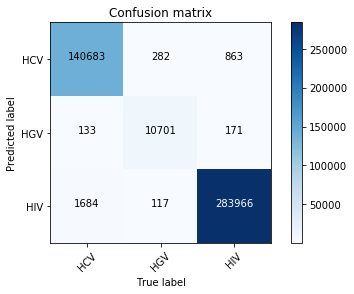
\includegraphics[width = .5\textwidth]{cm_k10.png}
		\caption{Confusion Matrix with k = 10}
		\label{fig6}
	\end{figure}
	For k = 10:\\
	For 438601 reads we generate 21902 clusters\\
	99.19\% HCV reads classfied into right clusters (HCV dominated cluster)\\
	97.24\% HGV reads classfied into right clusters (HGV dominated cluster)\\
	99.37\% HIV reads classfied into right clusters (HIV dominated cluster)\\
	
	\item 
	
	\begin{figure}[H]
		\centering
		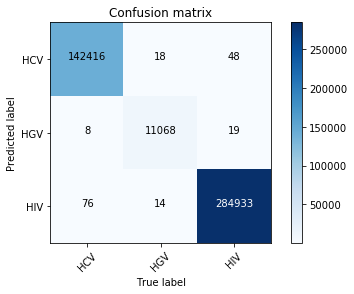
\includegraphics[width = .5\textwidth]{cm_k12.png}
		\caption{Confusion Matrix with k = 12}
		\label{fig7}
	\end{figure}
	For k = 12:\\
	For 438601 reads we generate 26819 clusters\\
	99.95\% HCV reads classfied into right clusters (HCV dominated cluster)\\
	99.76\% HGV reads classfied into right clusters (HGV dominated cluster)\\
	99.97\% HIV reads classfied into right clusters (HIV dominated cluster)\\
\end{enumerate}

We can see, if k is too small, then our cluster cannot distinguish the difference of three viral, as the kmer may not have enough variations. When we increase k, the classification error is smaller (as larger kmer can catch the signature information of that species) , but also we have much more clusters.

If our goal is to cluster all the reads into right clusters. Then it may be wise to choose larger k as beginning. Then later on we can merge small clusters to generate big clusters.
\end{document}
